%Przykładowy plik ułatwiający złożenie projektu dyplomowego inżynierskiego.
%UWAGA: Generowany napis na stronie tytułowej o treści PROJEKT DYPLOMOWY INŻYNIERSKI został zaproponowany przeze mnie i nie jest, póki co, potwierdzony przez władze wydziału. Przed ostatecznym oddaniem tak złożonej pracy należy upewnić się jaka powinna być treść tego napisu. W momencie gdy uzyskam informację na temat treści tego napisu, dokonam niezbędnych zmian w źródłach.

\documentclass[eng,printmode]{mgr}
%opcje klasy dokumentu mgr.cls zostały opisane w dołączonej instrukcji

%poniżej deklaracje użycia pakietów, usunąć to co jest niepotrzebne
\usepackage{polski} %przydatne podczas składania dokumentów w j. polskim
\usepackage[utf8]{inputenc} %kodowanie znaków, zależne od systemu
\usepackage[T1]{fontenc} %poprawne składanie polskich czcionek
\usepackage{url}
%pakiety do grafiki
\usepackage{graphicx}
\usepackage{subfigure}
\usepackage{psfrag}
% \usepackage{color}
% \usepackage{xcolor}
%pakiety dodające dużo dodatkowych poleceń matematycznych
\usepackage{amsmath}
\usepackage{amsfonts}
\usepackage{supertabular}
\usepackage{array}
\usepackage{tabularx}
\usepackage{hhline}

\usepackage{listings}		  %pozwalającyu listingować
\lstset{language=Python,      % sets automatic line breaking
 		numbers=left,
 		showstringspaces=false,
 		numbersep=5pt,
 		basicstyle=\tiny}

%pakiet wypisujący na marginesie etykiety równań i rysunków zdefiniowanych przez \label{}, chcąc wygenerować finalną wersję dokumentu wystarczy usunąć poniższą linię
\usepackage{showlabels}

%definicje własnych poleceń
\newcommand{\R}{I\!\!R} %symbol liczb rzeczywistych, działa tylko w trybie matematycznym
\newtheorem{theorem}{Twierdzenie}[section] %nowe otoczenie do składania twierdzeń

%dane do złożenia strony tytułowej
\title{Narzędzie do detekcji i ekstrakcji zdarzeń akustycznych w materiale audio}
\engtitle{A tool for detecting and extracting acoustic events in an audio material}
\author{Konrad Kamil Janowski}
\supervisor{dr Maciej Walczyński, Katedra Akustyki~i Multimediów (W4/K5)}

%\guardian{dr hab. inż. Imię Nazwisko Prof. PWr, I-6} %nie używać jeśli opiekun jest tą samą osobą co prowadzący pracę

%\date{2008} %standardowo u dołu strony tytułowej umieszczany jest bieżący rok, to polecenie pozwala wstawić dowolny rok


\field{Elektronika (EKA)}
\specialisation{Inżynieria akustyczna (EIA)}

%tutaj zaczyna się właściwa treść dokumentu
\begin{document}
\bibliographystyle{apalike} %tylko gdy używamy BibTeXa, ustawia polski styl bibliografii

\maketitle %polecenie generujące stronę tytułową
\dedication{6cm}{Dla rodziców, którzy zawsze mnie wspierali i~pozwolili mi rozwinąć się~w kierunku, który pragnąłem. Dziękuję.}

\tableofcontents %spis treści

\chapter{Wstęp}
\section{Cel i zakres pracy}
Przedmiotem pracy jest oprogramowanie do detekcji i~ekstrakcji zdarzeń akustycznych w materiale audio. Oprogramowanie zostało stworzone do obsługi plików w formacie wave o rozdzielczości bitowej szesnaście(16) i dwadzieścia cztery(24) bity oraz częstotliwości próbkowania czterdzieści cztery i sto dziesiątych (44,1) kilo Herca i~czterdzieści osiem (48) kilo Herca. Oprogramowanie zostało przetestowane używając plików o~tych parametrach. Oprogramowanie zostało stworzone modularnie aby możliwy był jego dalszy rozwój. Z~powodu tego założenia, program ma możliwość obsługi dowolnej częstotliwości próbkowania oraz dowolnej rozdzielczości bitowej choć nie jest to zalecane. Praca zawiera cztery moduły:
\begin{enumerate}
\item Moduł odczytywania pliku,
\item Moduł przetwarzania sygnału,
\item Moduł detekcji zdarzeń,
\item Moduł zapisu wyników do pliku.
\end{enumerate}
Autor ma nadzieję, że zaprojektowany w~ten sposób system pozwoli na późniejszy rozwój i~ułatwi powtórne wykorzystywanie tego narzędzia.
\section{Motywacja}
Analiza nagrań odgrywa bardzo ważną rolę we współczesnych zastosowaniach akustyki. Jednym z~przykładów może być ochrona ludzi przed hałasem. Aby zbadać hałas na stanowisku pracy lub ocenić narażenie na hałas przestrzeni publicznej niejednokrotnie wykonuje się bardzo długie nagrania, trwające nawet kilkanaście godzin. Ze względu na metody analizy nieraz niezbędne jest wyselekcjonowanie z~nagrania konkretnych zdarzeń akustycznych i~analiza ich w izolacji, nie biorąc pod uwagę poziomu tła w pozostałym czasie. 

Z~drugiej strony, możemy wyobrazić sobie potrzebę wyizolowania z~nagrania bardzo wielu zdarzeń akustycznych, które wydarzają się w krótkim odstępie czasu. Jako przykład może tutaj posłużyć strzelnica, gdzie chcąc policzyć liczbę strzałów w ciągu dnia możemy zrobić nagranie krótkie i~na podstawie tego krótkiego wycinka czasu oszacować hałas podczas całego dnia. Innym razem możemy mieć potrzebę wykryć te zdarzenia to celów z~pozoru nie związanych z~akustyką. Gdyby ktoś chciał policzyć ile razy została odbita piłka do koszykówki podczas badania jej wytrzymałości, jednym z~możliwych sposobów na zliczenie ilości odbić mogłoby być policzenie zdarzeń akustycznych jakimi są odbicia piłki od ziemi. Być może ktoś ze względów medycznych chciałby sprawdzić, ile czasu w~ciągu jego snu zajmuje chrapanie i~w ten sposób ocenić jak duży problem ma z~tą dolegliwością. Również w~tym przypadku, przy pewnej kontroli hałasu środowiska mógłby zrobić to za pomocą stworzonego narzędzia. Jak widać, wyszukiwanie zdarzeń akustycznych wraz z~czasem ich trwania może być niezwykle użyteczne w wielu z~pozoru nie związanych z~tym dziedzinach. 

Biorąc pod uwagę, że przytoczone wyżej przykłady są jedynie wąskim wycinkiem zastosowań, które mogłyby przyjść do głowy komuś, kto ma widzę i~zainteresowanie w~innej dziedzinie niż autor pracy nie ulega wątpliwości, że warto posiadać takie oprogramowanie. Oczywiście wszystkie przytoczone sytuacje można analizować ręcznie, odsłuchując nagrane próbki. Analiza takich nagrań jednak pochłania dużo czasu i może być problematyczna. Z~pomocą stworzonego narzędzia można proces zupełnie lub częściowo zautomatyzować co w~obu przypadkach skutkuje znaczną oszczędnością czasu. 

Praca powstała w połowie z~chęci stworzenia użytecznego narzędzia a~w~połowie z~chęci Autora do poznania współczesnych metod analizy cyfrowych sygnałów fonicznych. Rozwinięcie wiedzy w zakresie tworzenia oprogramowania w~języki Python, pracy z~systemem kontroli wersji oraz implementacja algorytmów znanych z~książek do realnie działającego programu jest procesem, który autor chciał zgłębić. Przedstawienie wyników w~formie zrozumiałej, czytelnej i~praktycznej jest nieraz jeszcze większym wyzwaniem i~nie można nabyć~w tym wprawy inaczej, niż pracując z~tymi wynikami i~samemu przekonać się na ile są one użyteczne.

Powyższe przesłanki zadecydowały o~stworzeniu narzędzia. 

\chapter{Wprowadzenie}
W tym rozdziale zostaną wprowadzone podstawowe pojęcia, którymi autor posługiwał się podczas tworzenia pracy. Omówione zostaną teoretyczne podstawy problemu oraz ogólna struktura logiczna programu.
\section{Zdarzenie akustyczne}
Jak wspomniano w powyższym rozdziale, nie ma jednej ogólnej definicji zdarzenia akustycznego, które odnosi się do wszystkich dziedzin akustyki. Jedna z~możliwych definicji podana jest w~normie \cite{PN-ISO-1996-1:2006} dotyczącej akustyki środowiskowej. Zapis normatywny mówi:

\begin{quotation}
"Należy podawać czas trwania zdarzenia~w odniesieniu do pewnej cechy dźwięku, jak np, liczba przekroczeń pewnego ustalonego poziomu. 

Przykład: czas trwania zdarzenia można zdefiniować jako całkowity czas, w~którym poziom ciśnienia akustycznego mieści się w zakresie 10 dB maksymalnego poziomu ciśnienia akustycznego podczas zdarzenia."\cite{PN-ISO-1996-1:2006}
\end{quotation}

Biorąc pod uwagę przytoczone wcześniej możliwe zastosowania stworzonego oprogramowania powyższa definicja dobrze opisuje te sytuacje, które mają być detekowane. Ponadto, wykonanie oprogramowania, które rozpoznaje zdarzenia opisane w normie daje perspektywy na możliwości jego praktycznego zastosowania.
\section{Przyjęta definicja zdarzenia akustycznego}
W poprzedniej sekcji przytoczony został zapis normatywny, który opisuje zdarzenie akustyczne na potrzeby akustyki środowiskowej. Sugeruje on, żeby czas trwania zdarzenia akustycznego definiować jako całkowity czas, w~którym poziom ciśnienia akustycznego mieści się w~zakresie 10 dB maksymalnego poziomu ciśnienia akustycznego podczas zdarzenia. 
Nie można zapomnieć, że pomiary w~akustyce środowiskowej często wykonywane są przez długi czas. Dla przykładu, pomiar hałasu na stanowisku pracy może być wykonywany przez osiem godzin bez przerwy\cite{PN-ISO-9612:2014}. Plik z ośmiogodzinnych pomiarów może być monofoniczny, zapisany~w formacie wave~o częstotliwości próbkowania czterdziestu ośmiu kilo Herców(48 kHz) oraz rozdzielczości dwudziestu czterech bitów. Każda próbka takiego pliku zajmuje zatem dwadzieścia cztery bity w~pamięci a~każda sekunda zawiera czterdzieści osiem tysięcy próbek.\cite{Principles_of_digital_audio} Przy pomocy prostego wzoru możemy obliczyć jego rozmiar w pamięci komputera liczonej w bitach:
\begin{equation}
\text{rozdzielczość bitowa} * \text{częstotliwość próbkowania} * \text{długość pliku} = \text{rozmiar pliku}
\end{equation}
\begin{equation}
24\;[b] * 48000\;[\frac{1}{s}] * 8*60*60\;[s] = 24\;[b] * 48000 \;[\frac{1}{s}] * 28800\;[s] = 3.31776*10^{10} \;[b] 
\end{equation}

Po przeliczeniu tego na jednostki bardziej sprzyjające interpretacji wyniku, przybliżając że $$1GB \approx 8*10^9 [b]$$ otrzymamy:


\begin{equation}
\frac{3.31776*10^10\;[b]}{8*10^9\;[\frac{b}{GB}]} = 4,1472 [GB]
\end{equation}
Po dokonaniu takich obliczeń, można zauważyć, że przetwarzania takiego pliku nie jest zadaniem trywialnym. Jeżeli program wczytywałby cały plik do pamięci RAM, potrzebowałby on około czterech gigabajtów tej pamięci na samo obsłużenie pliku. Gdy dodamy do tego potrzebę pamięci operacyjnej dla samego programu, potrzeby systemu operacyjnego oraz innych aplikacji działających równolegle z~programem zauważamy problem w~postaci braku tych zasobów. Nowoczesne stacje robocze poradziłyby sobie z~takim obciążeniem, jednak należy pamiętać o~kilku rzeczach:
\begin{itemize}
\item Nie wszystkie firmy~i osoby fizyczne dysponują stacjami roboczymi, posiadającymi duże zasoby pamięci operacyjnej RAM,
\item plik może być dłuższy,
\item plik może zostać nagrany~z wyższą częstotliwością próbkowania,
\item może nastąpić potrzeba współdzielenia pamięci~z innymi programami bez możliwości ich wyłączenia.
\end{itemize}

Powyższe czynniki w głównej mierze skłoniły autora do tego aby swój program oprzeć~o przetwarzanie sygnału fragmentarycznie. Dokładny sposób działania programu zostanie omówiony w dalszej części pracy. Co istotne w tym punkcie, wracając do definicji przytoczonej w normie \cite{PN-ISO-1996-1:2006} zadaniem nietrywialnym jest osiągnąć jednocześnie obie te funkcjonalności:
\begin{enumerate}
\item Odczytywanie programu fragmentarycznie.
\item Zapamiętanie wszystkich poprzednich wartości próbek aby w razie potrzeby cofnąć się do poprzedniego fragmentu celem odnalezienia spadku poziomu~o 10 dB.
\end{enumerate}

Mając na uwadze powyższe przesłanki oraz możliwość późniejszego rozszerzania funkcjonalności programu, autor zadecydował się aby ograniczyć definicję zdarzenia akustycznego do definicji:

\begin{quote}
"Należy podawać czas trwania zdarzenia~w odniesieniu do pewnej cechy dźwięku, jak np, liczba przekroczeń pewnego ustalonego poziomu."\cite{PN-ISO-1996-1:2006}
\end{quote}

Powyższa definicja jest mniej praktyczna niż jej rozszerzona wersja. Wymaga ona wiedzy o~pewnych danych środowiska i~zdarzenia, jak np. poziom tła akustycznego oraz przewidywany poziom ciśnienia akustycznego generowany podczas zdarzenia. Pomimo świadomości tych ograniczeń autor postanowił zastosować tę uproszczoną definicję, aby program realizował fragmentaryczne przetwarzanie danych i~tym samym spełniał w~całości założenia pracy jednocześnie dając lepsze możliwości na jego rozwój w przyszłości. Autor ma nadzieję, że dodanie innego algorytmu do detekcji bazującego na przetwarzaniu sygnału partiami będzie prostsze niż przyszła zmiana samego centrum oprogramowania, czyli odczytywania i~zapisywania wyników. 

\section{Metoda wykrywania zakłóceń}

Na podstawie informacji,~o których mowa powyżej autor podjął decyzję aby wykrywać przekroczenia pewnego ustalonego poziomu ciśnienia akustycznego. Ciśnienie akustyczne to jednak określenie zbyt ubogie aby w pełni precyzyjnie opisać funkcjonalność narzędzia. 
\section{Istniejące rozwiązania do wykrywania zdarzeń akustycznych}
\chapter{Metodologia}
W tej części zostanie omówiona metodologa przeprowadzonej pracy. Przedstawione zostaną narzędzia użyte to stworzenia programu, oprogramowanie, środowisko programistyczne oraz język programowania.
\section{System kontroli wersji - Git, GitHub, GitKraken}
\subsection{System kontroli wersji}
We współczesnym świecie istnieje bardzo wiele języków programowania. Każdy z nich~oferuje nieco inne możliwości i~funkcjonalności. Niezależnie jednak od wybranego języka, niezwykle istotnym jest system kontroli wersji. 

Jednym z~najpopularniejszych współcześnie systemów kontroli wersji jest Git. System kontroli wersji oferuje możliwość ciągłego śledzenia zmian w kodzie programu bez potrzeby ręcznego zapisywania wielu wersji pliku.\cite{Git}. Problem wersjonowania oprogramowania jest znany od dawna i~jest jednym z~kluczowych zagadnień pracy nad programem, szczególnie kiedy pracuje się w~zespole. Gdy kilka osób pracuje nad jednym fragmentem kodu, wydaje się niemożliwe aby współpracować bez systemu kontroli wersji.

Pomimo iż praca dyplomowa inżynierska jest projektem jednoosobowym, system kontroli wersji spełnia swoją rolę i~w takim przypadku. Praca z~kodem jest nierozłącznie związana z~wielokrotnymi zmianami wcześniej wprowadzonych rozwiązań. Czasami wynika to z~faktu odkrycia nowych, lepszych rozwiązań. Bywają też przypadki, kiedy w zaawansowanym stadium pracy okaże się, że już na samym początku został popełniony błąd w~logice działania i~trzeba coś zmienić w~jedne funkcji. Często te zmiany wymagają powrotu do momentu pracy sprzed paru dni a nawet tygodni, ponieważ kolejne fragmenty kodu opierały swoje funkcjonowanie na działaniu tych wadliwych elementów. Nie jest możliwym pamiętanie wszystkich tych zmian i~płynny powrót do nich poprzez przepisanie kodu. W takiej sytuacji, system kontroli wersji jest niezawodnym narzędziem, które pomaga zorganizować rozwój oprogramowania. 

Dodatkowo nie można nie docenić możliwości porównywania wersji roboczej pliku z~dowolną wersją tego pliku przechowywaną na serwerze. Daje to możliwość ocenienia wprowadzonych zmian, zastanowienia się czy wszystkie były konieczne oraz odpowiedniego przypomnienia sobie od czego zaczynaliśmy. Wszystkie te elementy pozwalają pracować w sposób efektywny i uporządkowany.

Ostatnim ale na pewno nie najmniej ważnym elementem jest możliwość przechowywania całego programu na zdalnym serwerze. W dobie komputeryzacji bardzo często zdarza się, że pracujemy na kilku różnych urządzeniach nad tym samym projektem. Korzystając z tego udogodnienia nie występuje problem przenoszenia danych pomiędzy urządzeniami. Dodatkowo w razie utraty sprzętu postępy pracy nie zostają stracone.
 
Powyżej omówione aspekty jednoznacznie wskazują, że pracując nad oprogramowaniem, chcąc robić to w~sposób odpowiedzialny i~umożliwiający przyszłą współpracę korzystanie z systemu kontroli wersji jest nieodzownym elementem pracy. Dbanie o czystość i~przejrzystość wprowadzanych zmian również jest elementem, którym powinna cechować się dobrze wykonana praca. 

\subsection{Git}
Jak zostało powiedziane, autor zdecydował się na skorzystanie z Git'a jako systemu do kontroli wersji. Jest to bardzo popularny system. Oferuję prostotę obsługi, przejrzystość, dobrą możliwość współpracy w małych grupach. Dodatkowo twórcy Git'a oferują darmowe prywatne miejsca na serwerze do przechowywania danych. Dzięki temu gestowi oraz wymienionych wyżej zaletach autor zadecydował się wybrać właśnie ten system. 

\subsection{GitKraken}
Pomimo iż autor zadecydował się tworzyć oprogramowanie w ramach pracy dyplomowej inżynierskiej warto pamiętać o tym, że praca w przeznaczeniu jest skierowana do akustyków. W związku z tym poza efektywnością działania programu ważne jest też jego prostota i przejrzystość aby podczas pracy nad nim oraz przyszłej możliwej rozbudowy można skupiać się na istocie działania a nie odkrywaniu zawiłych sposobów obsługi oprogramowania towarzyszącego.

Git w wersji podstawowej jest dostarczany z~bardzo ubogim graficznym interfejsem użytkownika. Przykładowe okno zostało zaprezentowane na obrazie (\ref{git_gui})

\begin{figure}[hbtp]  
	\caption{Graficzny interfejs użytkownika GIT}
	\label{git_gui}   
	\centering
	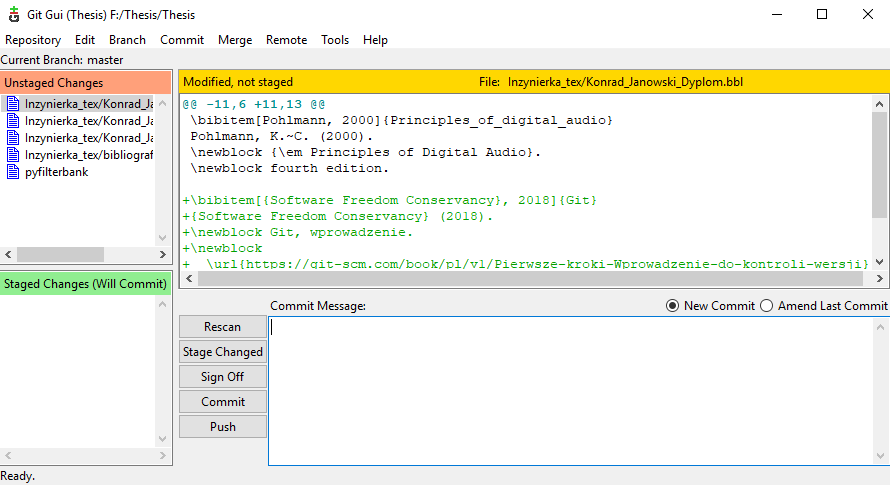
\includegraphics[width=0.8\textwidth]{git_gui.PNG}
\end{figure} 
 
Aby lepiej móc skupić się na logicznej strukturze programu autor zadecydował skorzystać z~programu GitKraken, który umożliwia pracę w~oparciu o system kontroli wersji Git w~bardziej przejrzystej i~czytelnej formie. Przykładowe drzewo kolejnych zmian zaprezentowano na obrazie (\ref{GitKraken})

\begin{figure}[hbtp]
\label{GitKraken}
\caption{Graficzny interfejs użytkownika programu GitKraken}
\centering
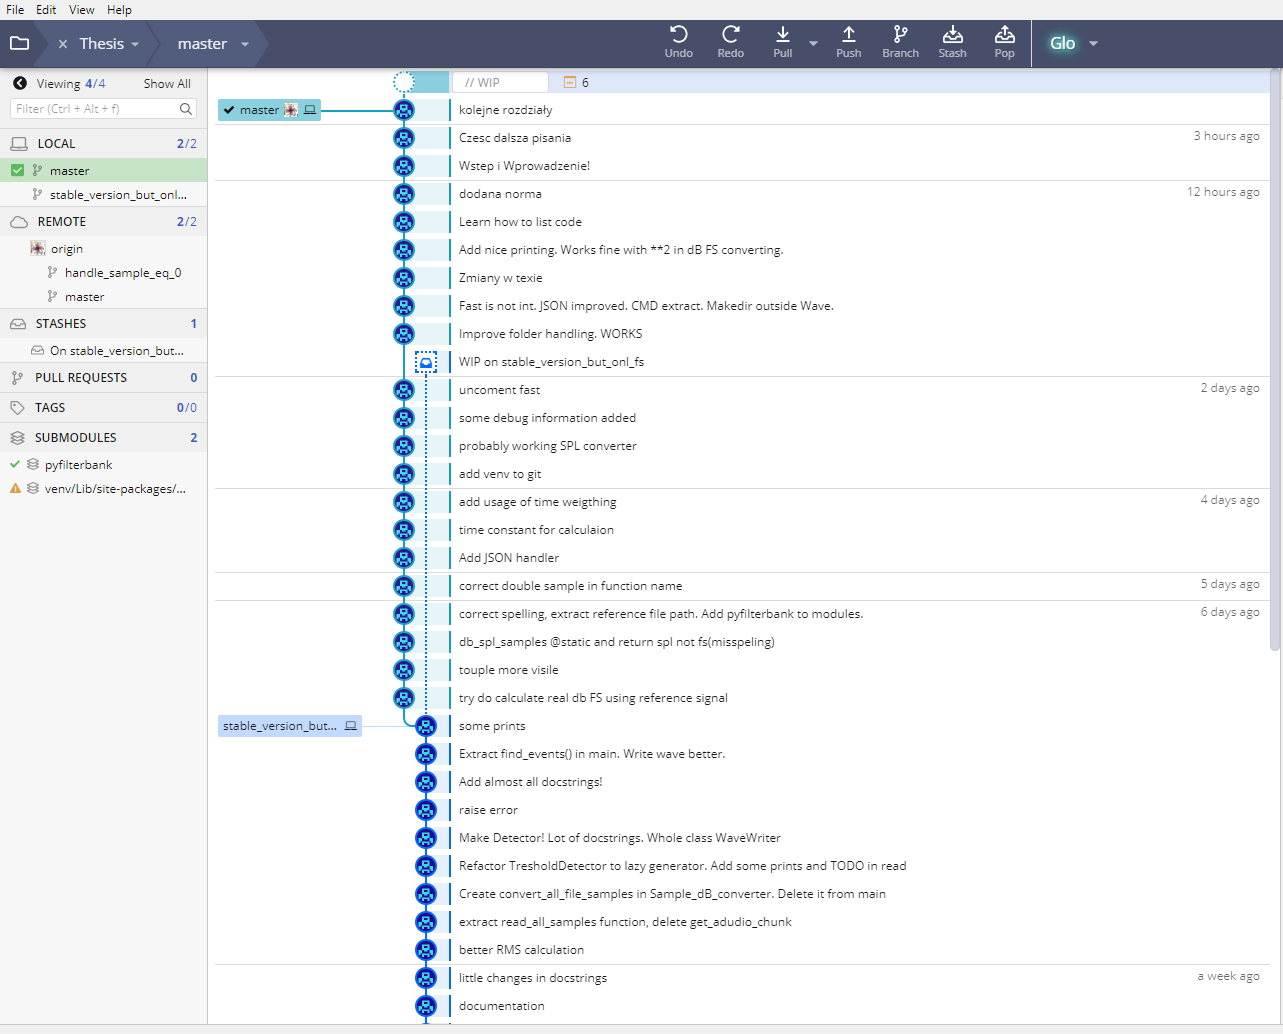
\includegraphics[width=0.8\textwidth]{GitKraken.PNG}
\end{figure}

W~opinii autora dobranie odpowiednich narzędzi jest bardzo istotne w~procesie tworzenia aplikacji. Wielu twórców oprogramowania, którzy nie są ukierunkowani na programowanie a~jedynie używają go jako narzędzia do wykonania innych czynności zaniedbuje wyżej wymienione aspekty dbałości o~czystość kodu. Dostęp i~odpowiednie użycie graficznych narzędzi, które są znacznie wygodniejsze i~bardziej intuicyjne niż ich konsolowe lub ubogie odpowiedniki z~pewnością może zachęcić twórców do większej dbałości o~ten aspekt tworzenia programów

\section{Język programowania - Python}
Mając pomysł na działanie programu oraz niezbędne narzędzie do kontrolowania postępów prac należy wybrac język programowania w~którym zostanie napisany program. Zdecydowano, że tym językiem będzie Python w wersji 3.7.1. Jest to najnowsza stabilna wersja tego języka\cite{Python_latest_release} w czasie tworzenia oprogramowania.

Wybrano Pythona z~kilku powodów. Python jest obecnie jednym z~najpopularniejszych języków programowania\cite{Python_popular}. Rozwijanie programu i przyszła współpraca z~innymi twórcami może być dzięki temu ułatwiona. Łatwiej znaleźć innych ludzi posługujących się Pythonem niż innymi, mniej popularnymi językami. 

Dodatkowo Python jest prosty w składni, intuicyjny i ma nieduży próg wejścia. Nawet osoba, która nie jest doświadczona w~programowaniu może stworzyć podstawowe aplikacje. Oczywiście bardziej zaawansowane struktury wymagają wiedzy, umiejętności i~ doświadczenia ale ta początkowa intuicyjność daje szansę zapoznania się z nim niezawodowym programistom.

Ponadto Python ma rozbudowaną bazę bibliotek i~modułów, które można używać ponownie do swoich zastosowań.\cite{Pypie} Daje to ogromne możliwości tworzenia programów dopasowanych do potrzeb, korzystając z~gotowych modułów. Gdyby za każdym razem trzeba było zapisywać podstawowe operacje od nowa, proces kodowania byłby zdecydowanie dłuższy i~mógłby zajmować więcej czasu niż osoba zajmująca się inną dziedziną może przeznaczyć na opracowanie narzędzia. 

Do tego Python ma doskonale opracowaną dokumentacje. Większość modułów jest opisana czytelnie i~zrozumiale. Zdecydowanie ułatwia to pracę z~tym językiem. 

Co ważne, Python jest językiem interpretowanym a nie kompilowanym.\cite{Przewodnik_po_pythonie}. Oznacza to, że do działania potrzebuje interpretatora, który działa niezależnie od systemu operacyjnego i jego bibliotek. Co prawda spowalnia to nieco jego działanie w porównaniu to języków kompilowanych takich jak C++ ale daje lepszą możliwość dzielenia się oprogramowaniem. Można skonstruować interpreter tak, by mógł być wysłany razem z kodem programu i osoba odbierająca bez problemu będzie mogła ten kod interpretować. W przypadku języków kompilowanych występują często problemu  z udostępnianiem kodu źródłowego właśnie ze względu na ich silna interakcję z systemem operacyjnym. W kontekście przyszłego rozwoju programu dla akustyków jest to ważny aspekt wyboru języka.

Z podanych powodów, Python został wybrany do napisania pracy.

Z wyborem Pythona wiąże się jeszcze jeden wybór, jego wersji. Obecnie najnowszą wersją jest Python 3.7.1 ale równocześnie wspierany jest Python w wersji 2.6.x.\cite{Python_latest_release}. Niestety, zmiana z~Pythona wersji drugiej na wersję trzecią wiąże się ze znaczącymi zmianami w~funkcjonalności języka i~wersje te nie są ze sobą kompatybilne. Wiele modułów aktualnie dostępnych do użytku dalej funkcjonuje w~wersji drugiej języka. Można by więc pokusić się o napisanie programu w starszej wersji. Python wersji drugiej przestaje jednak być wspierany wraz z końcem 2020 roku. \cite{Python_end_of_life}. Oznacza to, że najprawdopodobniej ze względów bezpieczeństwa i~braku wsparcia większość nowych modułów będzie pisana w~Pythonie w~wersji trzeciej a~dodatkowo w~razie nieprawidłowości w działaniu wersji drugiej, nie będzie można liczyć na żadną pomoc.


\section{Środowisko programistyczne - Pycharm}
Pycharm jest środowiskiem dedykowanym do obsługi Pythona. Mając niewielkie doświadczenie z~tym środowiskiem autor wybrał je aby je poznać i~sprawdzić jego działanie. Każde środowisko oferuje odmienny zestaw funkcjonalności i ułatwień użytkowania.
\chapter{Struktura oraz działanie programu}
\section{Struktura programu - aplikacja konsolowa}
Decydując się na program, należy wybrać w jaki sposób będzie on uruchamiany. Może być jedynie biblioteką, czyli zestawem funkcjonalności, które mogą być wykorzystywane przez inny program. Jest również możliwość skonstruowania rozbudowanego graficznego interfejsu użytkownika. Na ten moment, autor zadecydował aby oprogramowanie działało jako program konsolowy. 

Oznacza to, że wywołuje się go z konsoli systemu z odpowiednimi parametrami. Przykładowe wywołanie widzimy na obrazie(\ref{wywolanie})
\begin{figure}[hbtp]
\label{wywolanie}
\caption{Przykładowe wywołanie programu w konsoli systemu Windows}
\centering
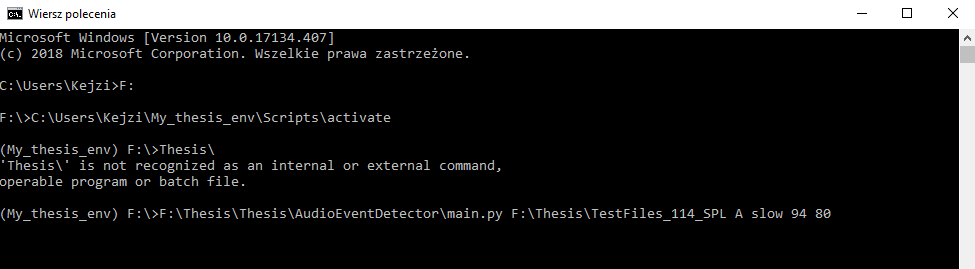
\includegraphics[width=0.8\textwidth]{cmd_wywolanie.PNG}
\end{figure}

\chapter{Notatki}
\begin{lstlisting}[frame=single]
\end{lstlisting}
\appendix
\chapter{Kod Programu}


\addcontentsline{toc}{chapter}{Bibliografia} %utworzenie w spisie treści pozycji Bibliografia
\bibliography{bibliografia} % wstawia bibliografię korzystając z pliku bibliografia.bib - dotyczy BibTeXa, jeżeli nie korzystamy z BibTeXa należy użyć otoczenia thebibliography

%opcjonalnie może się tu pojawić spis rysunków i tabel
% \listoffigures
% \listoftables
\end{document}
